\subsection{Blit}

\subsubsection{Descripción}

Esta operación recibe dos imagenes -original y blit- y genera una nueva combinando ambas. La combinación se realiza considerando un determinado color del blit como transparente para que en el resultado final algunos pixeles del blit queden por encima de la imagen original. En el lugar de aquellos que no son interpretados como transparentes quedan los pixeles del original. La imagen obtenida es una superposición de ambas, teniendo transparencias en el blit siempre que el color del pixel sea igual a (255,0,255).

% \begin{center}
% 	\begin{tabular}{cccc}
% 	  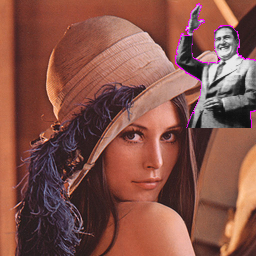
\includegraphics[width=0.2\textwidth]{imagenes/lenaBLIT.jpg} \\
% 	\end{tabular}
%    \end{center}

\begin{multicols}{2}
A pedido de la cátedra la imagen \textbf{blit} ser\'a una foto de Per\'on. La misma será ubicada en la esquina superior derecha de la imagen, además la imagen original deberá tener un tamaño mayor a 89 píxeles de ancho por 128 de alto para poder ubicar el blit. Como resultado tendremos una imagen \textit{Peronizada} cuando se aplique la siguiente función para cada p\'ixel $p$ en la imagen de Per\'on (blit):\\
\begin{center}
	\begin{tabular}{cccc}
	  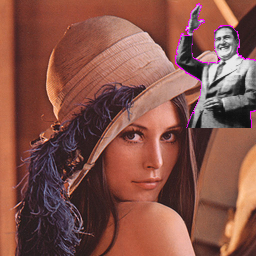
\includegraphics[width=0.3\textwidth]{imagenes/lenaBLIT.jpg} \\
	\end{tabular}
   \end{center}
\end{multicols}

$dst(p) = \begin{cases}
    src(p) & \mathrm{si \;} blit(p) \mathrm{\; es \; de \; color \; magenta, \; es \; decir \; sus \; colores \; son \;} (255, 0, 255)\\
    blit(p) & \mathrm{si \; no}
\end{cases}$ \\

\subsubsection{Implementación C}

% Es decir que si el p\'ixel en la imagen de Per\'on es magenta, entonces el nuevo p\'ixel tendr\'a los colores del p\'ixel correspondiente 
% en la imagen original; y si no los colores del p\'ixel en la imagen de Per\'on. \\

% Las columnas y filas que no se puedan procesar de esta manera, es decir, 
% las primeras $h - bh$ filas; y de las filas restantes, las primeras $w - bw$ columnas; 
% quedar\'an igual que como estaban originalmente. \\

Nuestra implementación en C consiste en dos etapas: primero copiamos los píxeles la imagen original en la imagen destino, luego copiamos los píxeles del blit siempre que los mismos no tengan el color (255,0,255). Como Perón debe estar arriba a la derecha de la imagen final, restamos el tamaño de su imagen al de la original en las dimensiones correspondientes. A continuación el pseudocódigo describe el algoritmo:

\begin{algorithm}[H]
  \begin{algorithmic}[1]
		\FORALL{y:=0 \TO  Height($I_{src}$)}		
			\FORALL{x:=0 \TO  Width($I_{src}$)}
			  \STATE $pixel \gets I_{src}(x,y)$ 
			  \STATE $I_{dst}(x,y) \gets pixel$
			\ENDFOR
		\ENDFOR
		\STATE $Int$ $ bh \gets $ Height($I_{src}$) $-$ Height($I_{blit}$)
		\STATE $Int$ $ bw \gets $ Width($I_{src}$) $-$ Width($I_{blit}$)
		 \FORALL{y:=0 \TO  Height($I_{blit}$)}
			\FORALL{x:=0 \TO  Width($I_{blit}$)}
			  	\STATE $pixel \gets I_{blit}(x,y)$
				\STATE $Int$ $ r \gets Red(pixel) $
			  	\STATE $Int$ $g \gets Green(pixel)$
			  	\STATE $Int$ $ b \gets Blue(pixel)$
				\IF{$\neg ( r = 255$ \AND $g = 0$ \AND $b=255)$}
					\STATE $I_{dst}(x+bw,y+bh) = I_{blit}(x+bw,y+bh)$ 
				\ENDIF
			\ENDFOR
		 \ENDFOR
  \end{algorithmic}
  \caption{$blit (I_{src}, I_{dst}, I_{blit})$}
  \label{alg:blit}
\end{algorithm}


\subsubsection{Implementación ASM}

En este filtro procesamos de a 4 píxeles: tenemos dos ciclos, uno que recorre las columnas de la imagen y otra que recorre las filas. Cuando nos encontramos en la fila "Height($I_{src}$) $-$ Height($I_{blit}$)" y la columna "Width($I_{src}$) $-$ Width($I_{blit}$)" es en este momento que tenemos que evaluar si aplicar o no el blit según la fórmula explicada arriba. Abajo detallaremos esta parte del código ASM que desarrolla el blit con un ejemplo.	

\begin{itemize}

	\item En los registros \textbf{xmm0,xnm14} tenemos la copia de los cuatro píxeles que levantamos de memoria, uno es $I_{src}$ y el otro $I_{blit}$ respectivamente.
			Y en \textbf{xnm2, xmm15} las máscaras que utilizamos para la comparación y las operaciones lógicas.

		\begin{center}
		   \begin{tabular}{| c | c | c | c || c | c | c | c || c | c | c | c || c | c | c | c |}
			 \hline
			 a & b & g & r & a & b & g & r & a & b & g & r & a & b & g & r \\ \hline
		   \end{tabular}
		   \\ \textbf{xmm0 $\gets$ $I_{src}$ }
		\end{center}

		\begin{center}
		   \begin{tabular}{| c | c | c | c || c | c | c | c || c | c | c | c || c | c | c | c |}
			 \hline
			 A & B & G & R & A & B & G & R & A & B & G & R & A & B & G & R \\ \hline
		   \end{tabular}
		   \\ \textbf{xmm14 $\gets$ $I_{blit}$ }
		\end{center}
		
		 
		\begin{center}
		   \begin{tabular}{| c | c | c | c || c | c | c | c || c | c | c | c || c | c | c | c |}
			 \hline
			 255 & 255 & 0 & 255 & 255 & 255 & 0 & 255 & 255 & 255 & 0 & 255 & 255 & 255 & 0 & 255 \\ \hline
		   \end{tabular}
		   \\  \textbf{Mascara Magenta xmm15 (maskMagenta)}
		\end{center}

		\begin{center}
		   \begin{tabular}{| c | c | c | c || c | c | c | c || c | c | c | c || c | c | c | c |}
			 \hline
			 00h & 00h & 00h & 00h & 00h & 00h & 00h & 00h & 00h & 00h & 00h & 00h & 00h & 00h & 00h & 00h \\ \hline
		   \end{tabular}
		   \\ \textbf{Mascara en xmm2 (maskCeros)}
		\end{center}
		
	\item Máscara para filtrar píxeles de valor magenta. Suponemos que hay dos píxeles color magenta en $I_{blit}$ a modo de ejemplo en los píxeles 1 y 3 (siguiendo el order de píxel_15,...,píxel_0). A esta máscara la guardamos en xmm12 y xmm15.
	
		\begin{center}
		   \begin{tabular}{| c | c | c | c || c | c | c | c || c | c | c | c || c | c | c | c |}
			 \hline
			 0xFF & 0xFF & 0xFF & 0xFF & 0x00 & 0x00 & 0x00 & 0x00 & 0xFF & 0xFF & 0xFF & 0xFF & 0x00 & 0x00 & 0x00 & 0x00 \\ \hline
		   \end{tabular}
		   \\ \textbf{xmm12,xmm15 $\gets$ pcmpeqd xmm15, xmm14}
		\end{center}

	\item Máscara para filtrar píxeles que no son magenta.

		\begin{center}
		   \begin{tabular}{| c | c | c | c || c | c | c | c || c | c | c | c || c | c | c | c |}
			 \hline
			 0x00 & 0x00 & 0x00 & 0x00 & 0xFF & 0xFF & 0xFF & 0xFF & 0x00 & 0x00 & 0x00 & 0x00 & 0xFF & 0xFF & 0xFF & 0xFF \\ \hline
		   \end{tabular}
		   \\ \textbf{xmm15 $\gets$ pcmpeqd xmm15, xmm13}
		\end{center}

	\item  Me quedo con los valores de $I_{src}$ que tengo que poner en la imagen $I_{dst}$.
		\begin{center}
		   \begin{tabular}{| c | c | c | c || c | c | c | c || c | c | c | c || c | c | c | c |}
			 \hline
			 A & B & G & R & 0x00 & 0x00 & 0x00 & 0x00 & A & B & G & R & 0x00 & 0x00 & 0x00 & 0x00 \\ \hline
		   \end{tabular}
		   \\ \textbf{xmm12 $\gets$ pand xmm12, xmm0}
		\end{center}		

	\item Me quedo con los valores de $I_{blit}$ que tengo que poner en la imagen $I_{dst}$.
		\begin{center}
		   \begin{tabular}{| c | c | c | c || c | c | c | c || c | c | c | c || c | c | c | c |}
			 \hline
			 0x00 & 0x00 & 0x00 & 0x00 & a & b & g & r & 0x00 & 0x00 & 0x00 & 0x00 & a & b & g & r \\ \hline
		   \end{tabular}
		   \\ \textbf{xmm15 $\gets$ pand xmm15, xmm14}
		\end{center}		
	
	\item Junto todos los valores en XMM15.
		\begin{center}
		   \begin{tabular}{| c | c | c | c || c | c | c | c || c | c | c | c || c | c | c | c |}
			 \hline
			 A & B & G & R & a & b & g & r & A & B & G & R & a & b & g & r \\ \hline
		   \end{tabular}
		   \\ \textbf{xmm15 $\gets$ por xmm15, xmm12}
		\end{center}		
	\item Por último resta guardar estos 4 píxeles (XMM15) en $I_{dst}$.

\end{itemize}

Para más detalles dejamos un extracto del código ASM:

\begin{codesnippet}
\begin{verbatim}
	maskMagenta: db 255	 ,0, 255, 255, 255, 0, 255, 255, 255, 0, 255, 255, 255, 0, 255, 255
	maskCero: db 0, 0, 0, 0, 0, 0, 0, 0, 0, 0, 0, 0, 0, 0, 0, 0 

section .text

blit_asm:
		...
		movdqu xmm0, [rdi]; xmm0=|A B G R|A B G R|A B G R|A B G R|; img	
		movdqu xmm14, [r15]; xmm14=|a b g r|a b g r|a b g r|a b g r|; blit
							   ;Filtro los valores color magenta
		pcmpeqd xmm15, xmm14   ; xmm15=|FF FF FF FF|00 00 00 00|FF FF FF FF|00 00 00 00| 
		movdqu xmm12, xmm15	   ; xmm12= xmm15 paso la mascara a xmm12 
							   ;Filtro los valores que no son magenta
		pcmpeqd xmm15, xmm13   ; xmm15=|00 00 00 00|FF FF FF FF|00 00 00 00|FF FF FF FF|
							   ;Me quedo con los velores de xmm0 que tengo que poner en la imagen
		pand xmm12, xmm0       ; xmm2=|A B G R|00 00 00 00|A B G R|00 00 00 00|
							   ;Me quedo con los valores de blit que tengo que poner en la imagen
		pand xmm15, xmm14      ; xmm15=|00 00 00 00|a b g r|00 00 00 00|a b g r|
							   ; Junto los dos valores en xmm15
		por xmm15, xmm12 	   ;xmm15=|A B G R|a b g r|A B G R|a b g r|
		movdqu [rsi], xmm15	   ; Copio todo a dst
		movdqu xmm15, [maskMagenta]
		movdqu xmm13, [maskCero]
		...
\end{verbatim}
\end{codesnippet}